\chapter{Wykład 9. Zarządzanie czasem w projekcie informatycznym}

\section{SPP uwzglęniający plan kont kosztowych projektu}
% strona 34

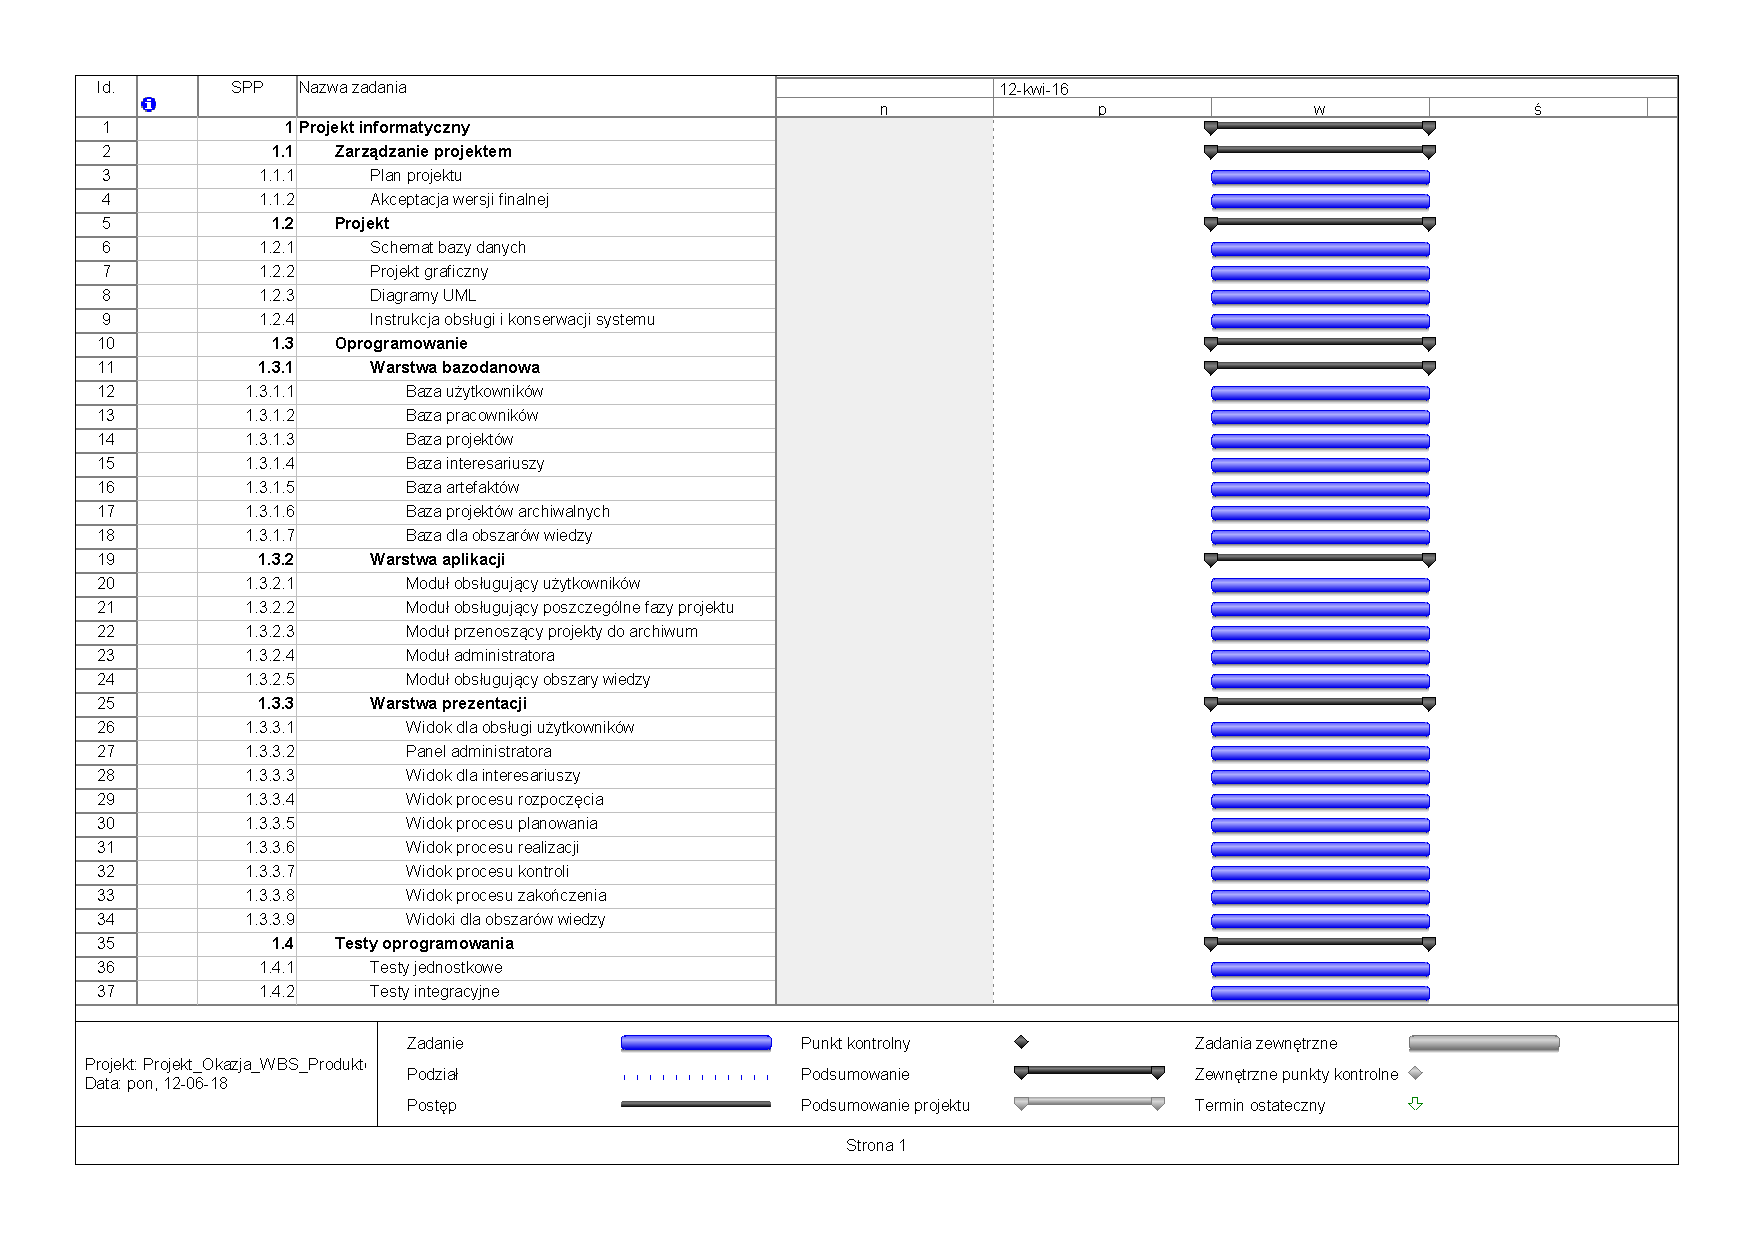
\includepdf[nup=1x2,pages=-]{diagramSPP.pdf}

% ===========================================================================

\section{Harmonogram w MS Project}
% strona 35

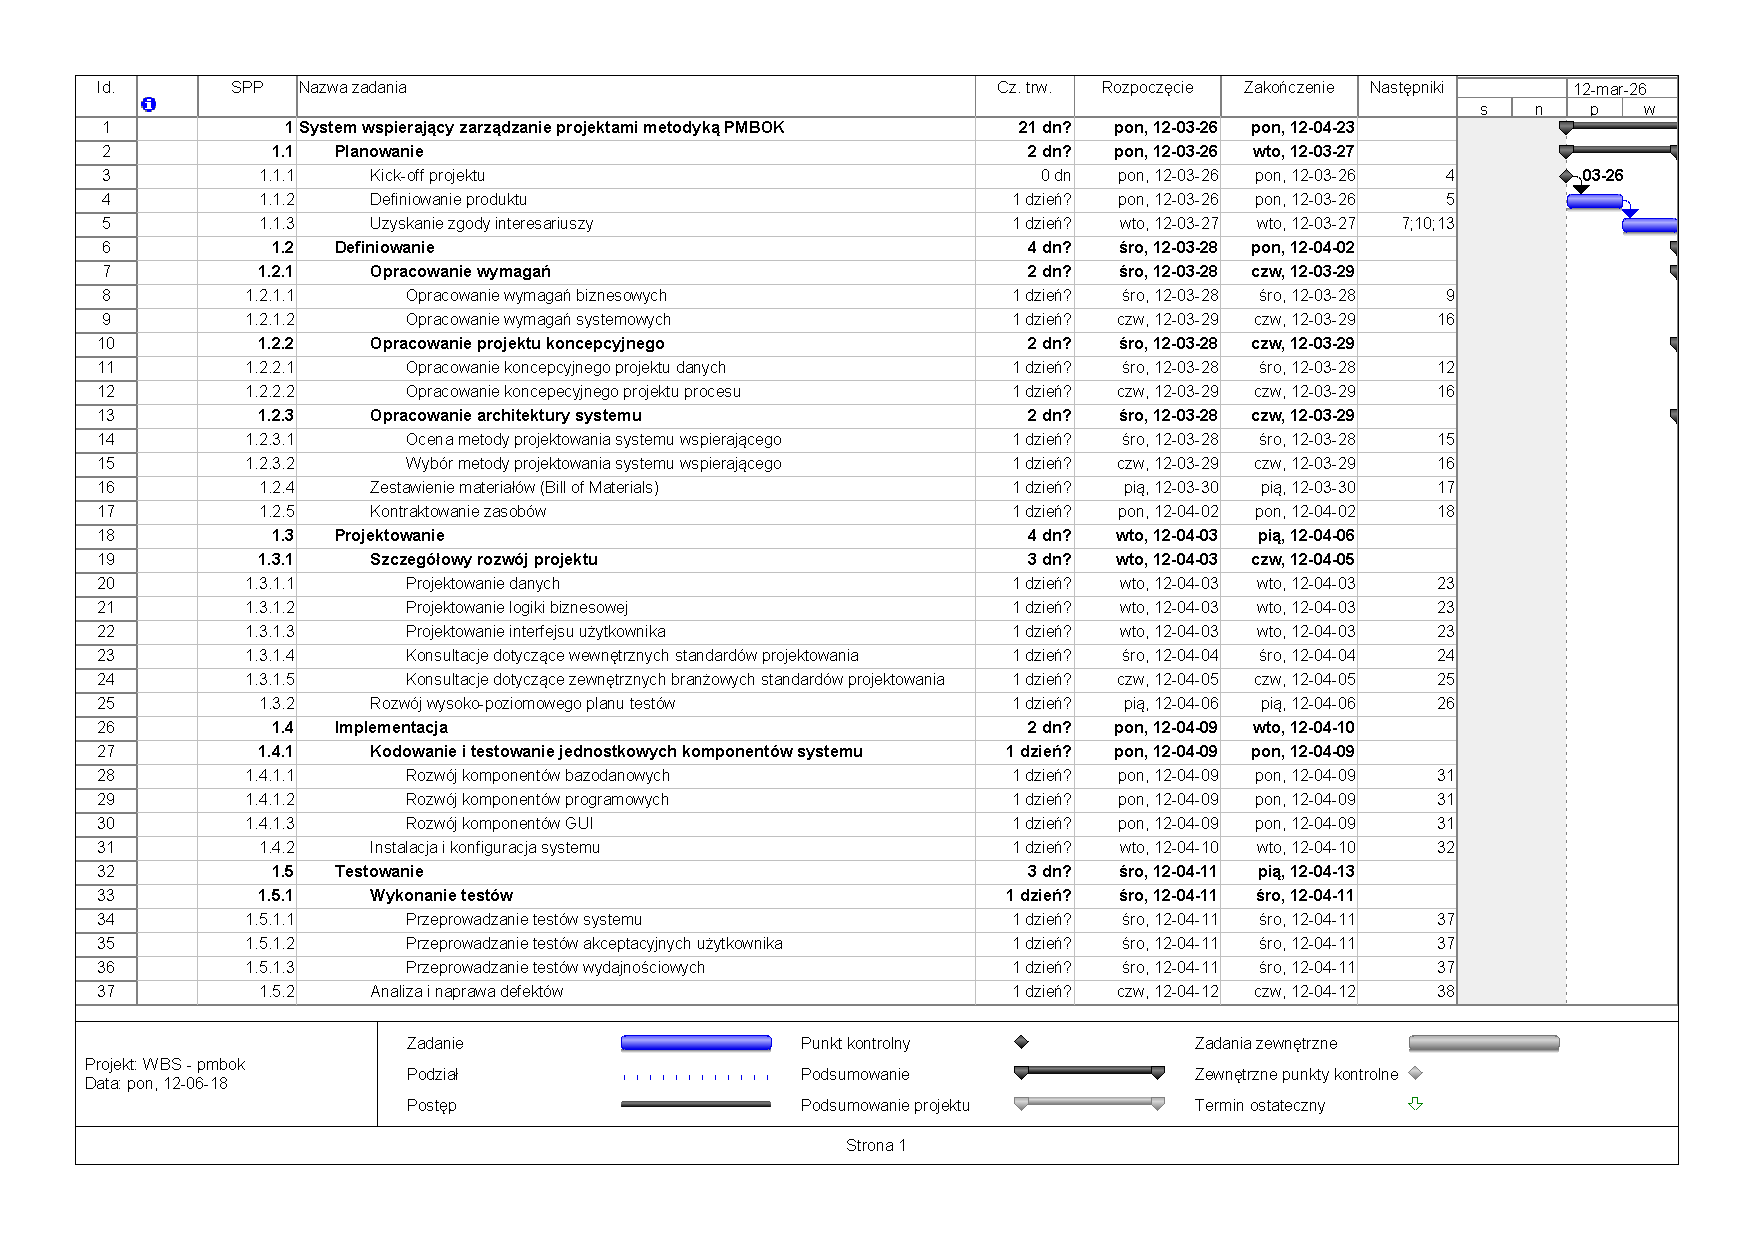
\includepdf[nup=2x2,pages=-,landscape=true,column=true]{harmonogramWBS.pdf}

% ===========================================================================

\begin{landscape}

\section{Struktura RBS projektu}
% strona 45

\begin{figure}[!h]
\centering
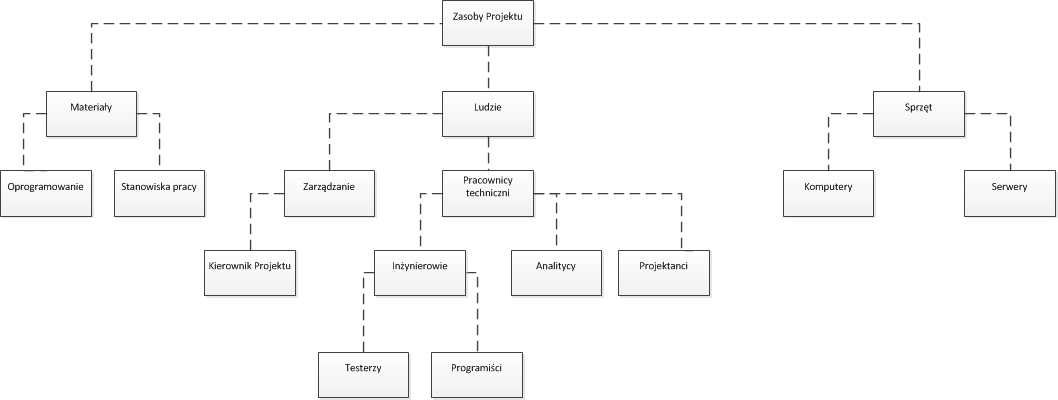
\includegraphics[width=1.5\textwidth]{RBS.png}
\caption[RBS]{RBS}
\label{rysunekProces}
\end{figure}

\end{landscape}

% ===========================================================================

\section{Harmonogram z uwzględnieniem zasobów}
% strona 59

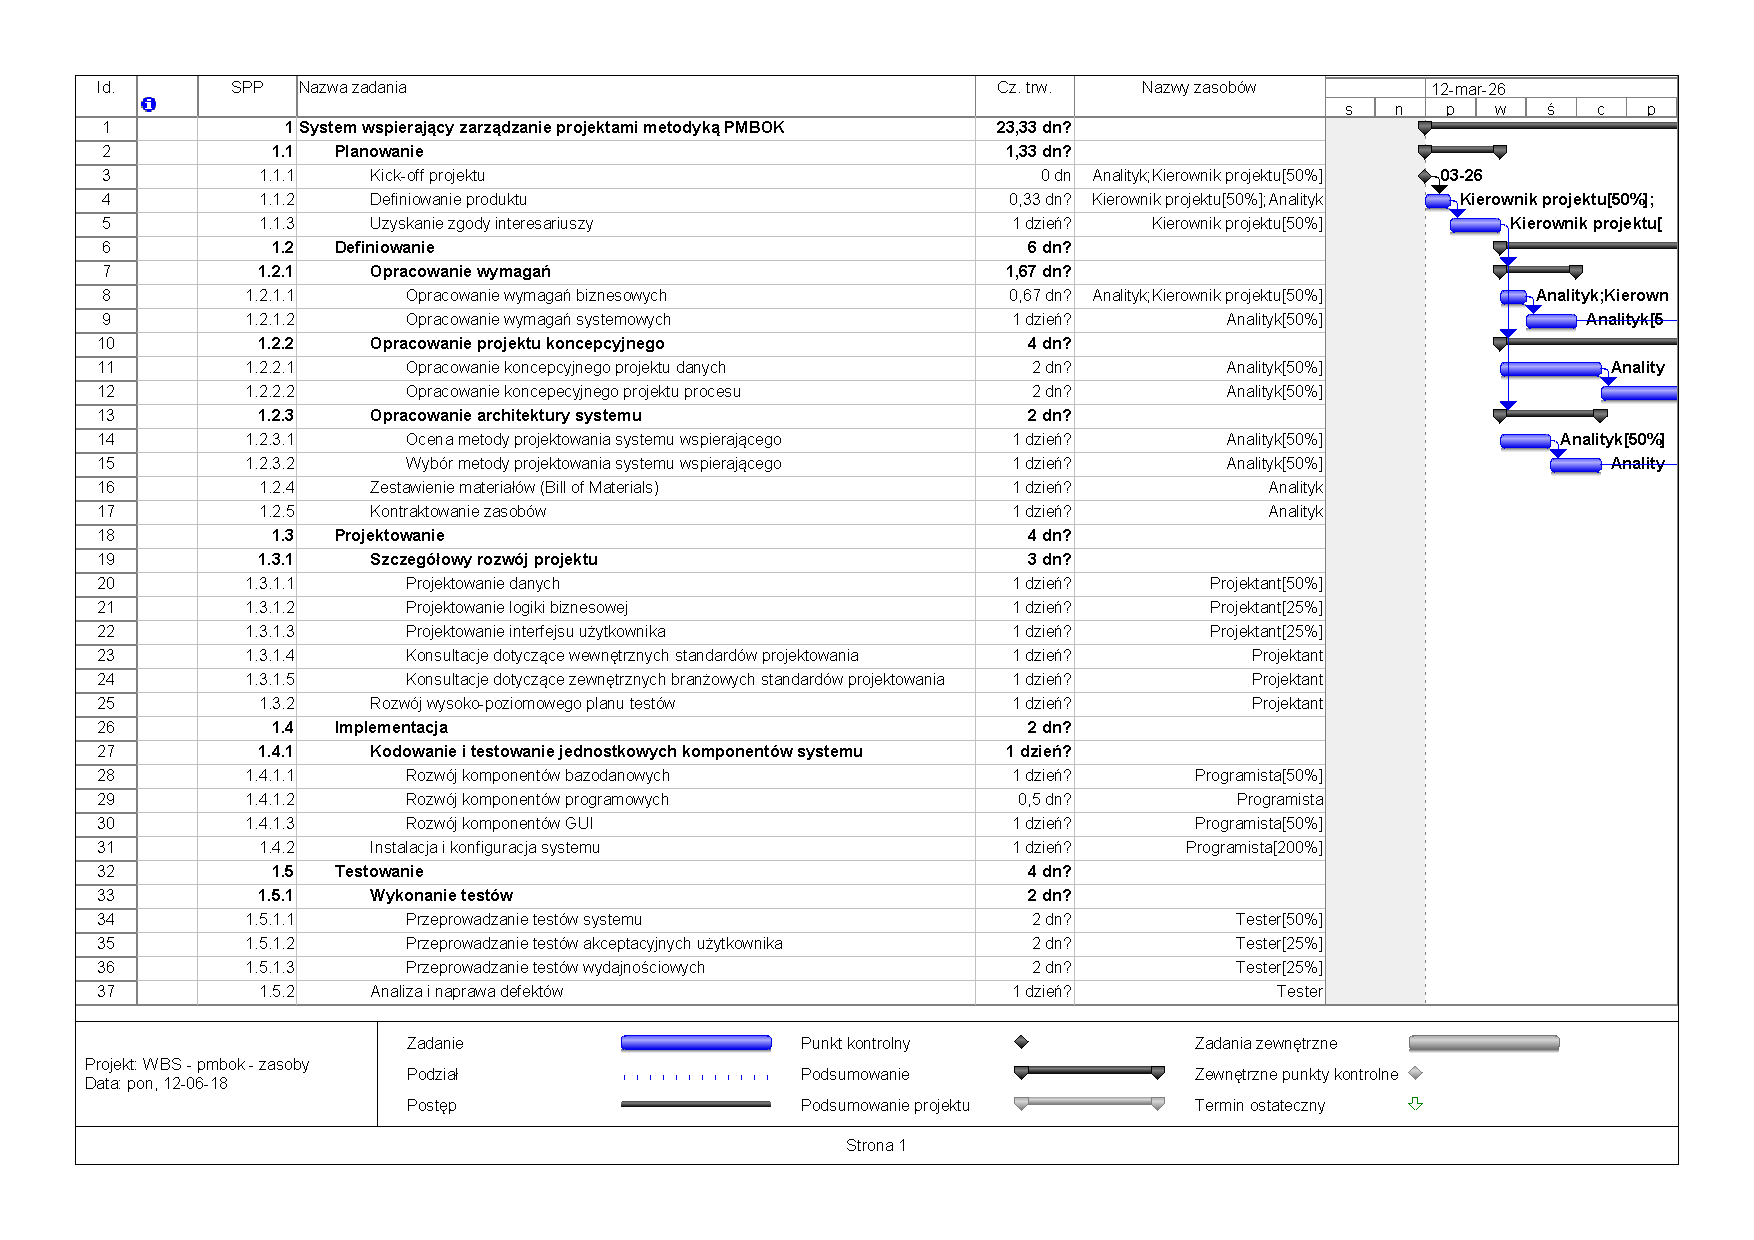
\includepdf[nup=2x2,pages=-,landscape=true,column=true]{zasobyWBS.pdf}

